\documentclass{beamer}
\usepackage{beamerthemeshadow}
\usepackage{graphicx}
\usepackage{color}
\usepackage[utf8]{inputenc}
\usepackage[T1]{fontenc}
\usepackage{hyperref}
\usepackage{caption}
\usepackage[flushleft]{threeparttable}
\usepackage{subfigure}

\definecolor{cerulean}{HTML}{005776} 
\setbeamercolor{structure}{fg=cerulean}
\captionsetup[figure]{labelformat=empty}
\captionsetup[table]{labelformat=empty}


\def\d{{\fontencoding{T1}\selectfont\dj}}
\def\D{{\fontencoding{T1}\selectfont\DJ}}


\title{Kvantna kriptografija}
\subtitle{Tehničko i naučno pisanje}

\makeatletter
\long\def\beamer@author[#1]#2{%
  \def\and{\tabularnewline}
  \def\insertauthor{\def\inst{\beamer@insttitle}\def\and{\tabularnewline}%
  \begin{tabular}{rl}#2\end{tabular}}%
  \def\beamer@shortauthor{#1}%
  \ifbeamer@autopdfinfo%
    \def\beamer@andstripped{}%
    \beamer@stripands#1 \and\relax
    {\let\inst=\@gobble\let\thanks=\@gobble\def\and{, }\hypersetup{pdfauthor={\beamer@andstripped}}}
  \fi%
}
\makeatother

\author[I. Glišović \and Ž. Zekavičić \and N. Lazarević \and A. Mladenović]{%
*Igor Glišović, &  \it{mi22292@alas.matf.bg.ac.rs}\and
Željko Zekavičić, &  \it{mi22130@alas.matf.bg.ac.rs}\and
Nađa Lazarević, &  \it{mi22175@alas.matf.bg.ac.rs}\and
Ana Mladenović, &  \it{mi22119@alas.matf.bg.ac.rs}
}
\institute{Matematički fakultet\\Univerzitet u Beogradu}
\date{
	\footnotesize{Beograd, 2022.}	
}

\begin{document}
\transdissolve
\begin{frame}
	\thispagestyle{empty}
	\titlepage
\end{frame}

\addtocounter{framenumber}{-1}

\begin{frame}[fragile]\frametitle{Literatura}
	\begin{itemize}
		\item Zasnovano na seminarskom radu:\\
		\it{\href{https://github.com/zeljkozekavicic/28_TNP2022/blob/main/28_GlisovicZekavicicLazarevicMladenovic.pdf}{Kvantna kriptografija; Igor Glišović, Željko Zekavičić,\\Nađa Lazarević, Ana Mladenović}}
  
	\end{itemize}
\end{frame}



\section{Uvod}

\begin{frame}[fragile]
\transdissolve
\frametitle{Uvod}
	\begin{itemize}
	    \item Kriptografija - očuvanje tajnosti podataka
        \item Razvoj klasične kriptografije - OneTimePad
        \item Problem moderne kriptografije: \bf{"Kvaka 22"}
	\end{itemize}
 \bigskip
 \begin{centering}
    \emph{
    Komunikacija između pošiljaoca i primaoca je sigurna\\ $\iff$ \\  Kriptografski sistem je 
    siguran
 
    }
 \end{centering}
 \transdissolve
\end{frame}

\section{Istorijat}



\begin{frame}[fragile]

\frametitle{Istorijat}
\bigskip
	\begin{itemize}	
		\item Sigurna komunikacija - pitanje sve od praistorije pa do XX veka
		\item Stephen Weisner - tvorac kvantne kriptografije
      \item C.H.Bennet, G. Brassard - kvantna kriptografija na delu
      \item Arthur Ekert - kvantna isprepletanost
	\end{itemize}
 \begin{figure}[h!]
        \centering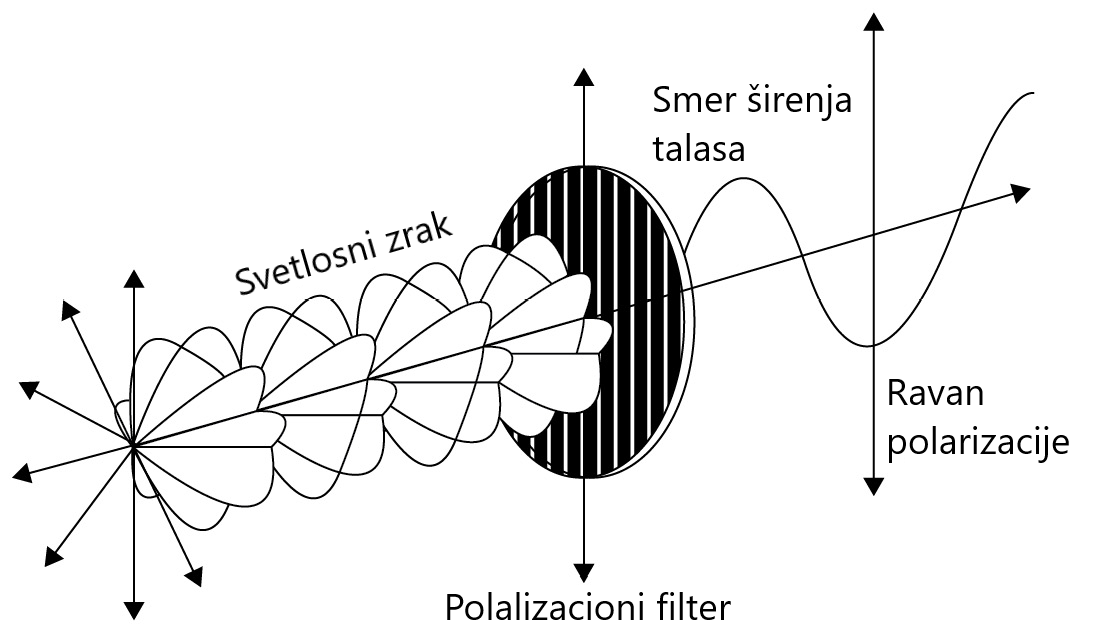
\includegraphics[height=3cm]{sl2.png} 
        \caption{Slika 1: \emph{Polarizacija fotona - osnova \\kvantne kriprografije}}
        \label{fig:polarizacija}
        \end{figure}
        
 
\end{frame}

\section{Principi kvantne kriptografije}

\subsection{Kvantna mehanika, kvantni računari}

\begin{frame}[fragile]\frametitle{Kvantna mehanika, kvantni računari}\bigskip
	\begin{itemize}	
		\item Aspekti kvantne mehanike
            \begin{itemize}
                \item aspekt prirodne neodređenosti
                \item aspekt kvantnog sprezanja
                \item uticaj međusobnog delovanja čestica
            \end{itemize}
		\item Osnova kvantnih računara - kvantni biti, \bf{kubiti}
	\end{itemize}
 \bigskip
        \begin{figure}[h!]
        \centering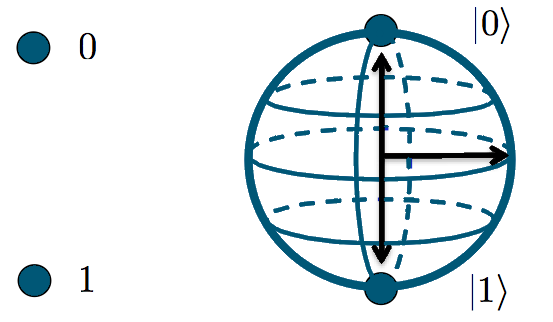
\includegraphics[height=2cm]{sl1.png} 
        \caption{Slika 2: \emph{bit (levo), kubit (desno)}}
        \label{fig:bitkubit}
        \end{figure}
 
\end{frame}

\subsection{Kvantni protokoli, kvantna razmena ključa}
\begin{frame}[fragile]\frametitle{Kvantni protokoli, kvantna razmena ključa}
\bigskip
	\begin{itemize}	
		\item Distribucija kvantnih ključeva (\textit{QKD - Quantum Key Distribution}) i različiti protokoli
        \begin{itemize}
            \item BB84 protokol ("pripremi i izmeri")
                
            \item E91 protokol (isprepletanost kubita)
            
        \end{itemize}
	\end{itemize}
 \smallskip
        \begin{figure}[h!]
        \centering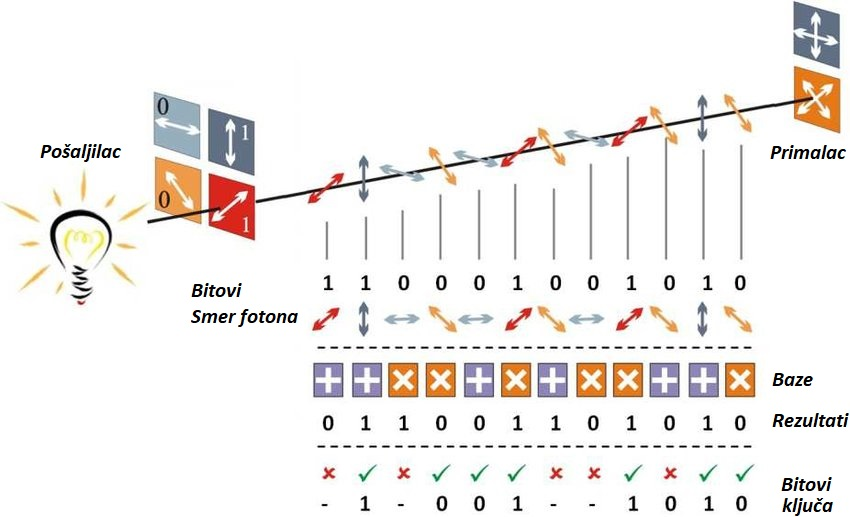
\includegraphics[height=3cm]{bb84.jpg} 
        \caption{Slika 3: \emph{Metodika rada BB84 protokola}}
        \label{fig:bb84}
        \end{figure}
 
\end{frame}

\subsection{Vrste napada na sistem i odbrana}
\begin{frame}[fragile]\frametitle{Vrste napada na sistem i odbrana}
\bigskip
	\begin{itemize}	
	  \item Nekoliko vrsta napada na kriptografske sisteme:
        \begin{itemize}
            \item "Middleman" napad
            \item PNS (photon-number splitting) napad
            \item Hakerski napad
            \item DOS (denial of service) napad
        \end{itemize}
        \item Zaštitu obezbeđujemo\bf{ sigurnim i pouzdanim sistemom} 
        
	\end{itemize}
    \begin{figure}[h!]
        \centering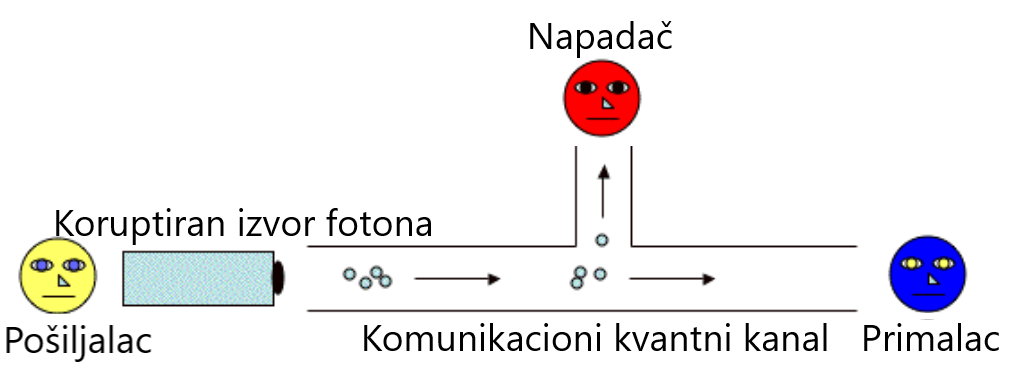
\includegraphics[height=2cm]{sl3.png} 
        \caption{Slika 4: \emph{PNS napadač iskorišćava slabost sistema}}
        \label{fig:pns}
        \end{figure}
\end{frame}

\section{Implementacija kvantne kriptografije}
\begin{frame}[fragile]\frametitle{Implementacija kvantne kriptografije}
	\begin{itemize}
	    \item Što je veća udaljenost slanja - nesigurniji je sistem
        \item Kineski istraživači - "pouzdani" relejni čvorovi
        \item Shorov algoritam za faktorizaciju brojeva
	\end{itemize}
 {\scriptsize
\begin{table}[h]
\centering
\begin{tabular}{|l|c|}
\hline
\textbf{Naziv i godina projekta}                           & \textbf{Dužina prenosa} \\ \hline
Prenos novca Creditanstalt banke, Austrija 2004.           & 1.45 km                 \\ \hline
IdQuantique i Deckpoint kolaboracija, Švajcarska 2005.     & 10 km                   \\ \hline
Povezivanje Kanarskih ostrva, Španija 2006.                & 144 km                  \\ \hline
SECOQC, prvi kvantno-kriptografski računar, Austrija 2008. & 200 km                  \\ \hline
\end{tabular}
\caption{Tabela 1: \emph{Razvoj dužine prenosa kvantno-kriptografskih sistema}}

\label{tabela:kvantnaxxii}
\end{table}
}
\end{frame}

\section{Zaključak}

\begin{frame}[fragile]\frametitle{Zaključak}
\bigskip
	\begin{itemize}
        \item Veoma sigurni sistemi koji se razvijaju i danas
        \item Šira primena je trenutno nemoguća zbog \textbf{cene implementacije} potrebne infrastrukture
	    \item Primena kvantne kriptografije u budućnosti je izvesna
	\end{itemize}
    \begin{figure}[h!]
        \centering
        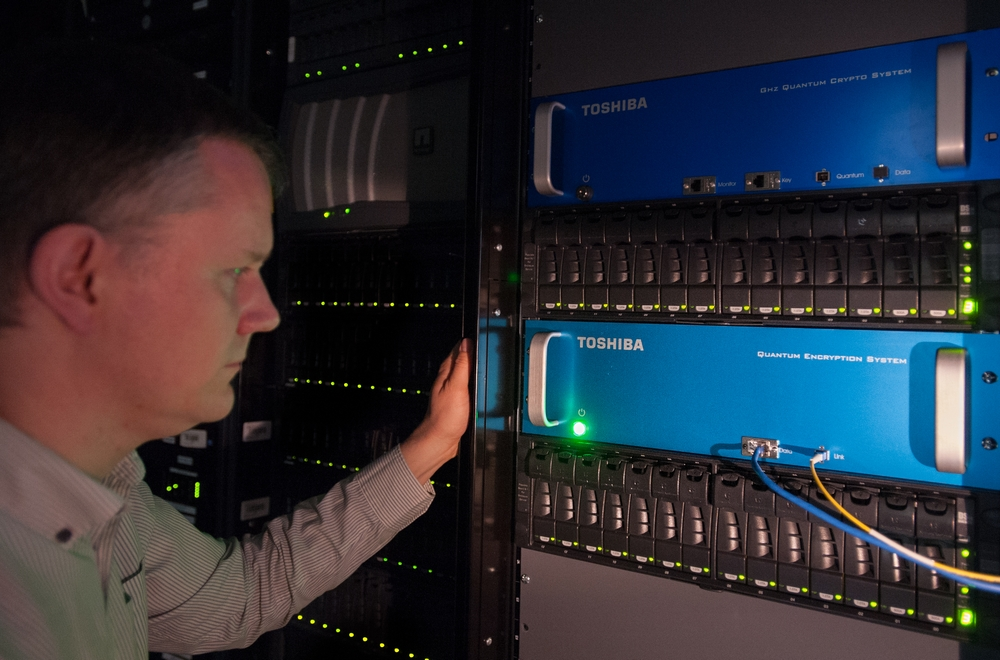
\includegraphics[height=3cm]{sl4.jpeg} 
        \caption{Slika 5: \centering{\emph{"Luksuz" korišćenja ovakvih sistema sada mogu priuštiti samo najimućnije firme, poput Toshibe}}}
        \label{fig:toshiba}
        \end{figure}
\end{frame}

\end{document}
